% !TEX root = ../main.tex

\newpage
\section{Related work}
Several solutions have been proposed by Ethereum community---mostly from developers on GitHub\cite{Ref07}---to address the attack. There would be some trad-offs for each solution that needs to be evaluated in term of conforming with standard constraints and attack mitigation. We have examined mitigation approach of each solution and explained possible ERC20 constraint violation.

\subsection{Enforcement by User Interface (UI)}
ERC20 standard recommends to set allowance to zero before any non-zero values and enforce approval processing check in UI instead of smart contract:
\begin{figure}[t!]
	\centering
	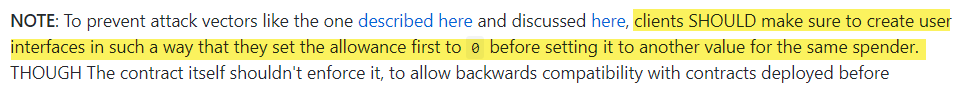
\includegraphics[width=1.0\linewidth]{figures/multiple_withdrawal_03.png}
	\caption{Recommendation of ERC20 standard to mitigate multiple withdrawal attack by enforcement in UI.}
\end{figure}


\noindent If Alice does not use UI and connects directly to the blockchain, there would be a good chance of impacting by this attack. Even if she uses UI, this approach can not prevent the attack. As discussed on GitHub\cite{Ref14}, Bob still can transfer N+M tokens in the below scenario:
\begin{enumerate}
	\item Bob is allowed to transfer N Alice’s tokens.
	\item Alice publishes a new transaction that changes Bob’s allowance from N to 0.
	\item Bob front runs Alice’s transaction and transfers N Alice’s tokens (\textit{transferFrom} sets Bob’s allowance to 0 respectively).
	\item Alice’s transaction is mined and sets Bob’s allowance to 0.
	\item Now Alice publishes a new transaction that changes Bob’s allowance from 0 to M.
	\item Alice’s second transaction is mined, Bob now is allowed to move M Alice’s tokens.
	\item Bob transfers M Alice’s tokens and in total N+M.\newline
\end{enumerate}
At step 3, Bob is able to transfer N tokens and consequently his allowance becomes 0 by \textit{transferFrom} method. This is considered as a legitimate transaction since Alice has already approved it. The issue occurs after Alice’s new transaction in step 5 to set Bob's allowance to M. In case of front-running by Bob, Alice needs to check Bob’s allowance for the second time before setting any new value. However, she finds out Bob’s allowance 0 in either case. In other words, she can not distinguish whether Bob’s allowance is set to 0 because of her transaction in step 2 or Bob already transferred tokens by front-running is step 3 and that made his allowance 0. Someone may point out that Alice notices this by checking \textit{Transfer} event logged by \textit{transferFrom} function. However, if Bob had transferred tokens to someone else (like Carol), then \textit{Transfer} event will not be linked to Bob, and, if Alice’s account is busy and many people are allowed to transfer from it, Alice may not be able to distinguish this transfer from a legitimate one performed by someone else. Overall, this solution does not prevent the attack while tries to follow ERC20 recommendations for setting Bob’s allowance to zero before any non-zero value. Hence, enforcement should be considered at contract level not UI to remove the gap between transactions and mitigate the attack. Interestingly, OpenZeppelin example implements a workaround in contract level that makes it inconsistent with the recommendations of ERC20. 

\subsection{Minimum viable token}
As suggested by Ethereum Foundation\cite{Ref05}, we can boil down ERC20 standard to a very basic functionalities by implementing only essential methods. this will prevent effecting of the attack by skipping implementation of vulnerable functions. While removing \textit{approve} and \textit{transferFrom} functions prevent the attack, it makes the token partially-ERC20-compliant. Golem Network Token (GNT\footnote{https://etherscan.io/address/0xa74476443119A942dE498590Fe1f2454d7\newline D4aC0d\#code}) is one of these examples since it does not implement the \textit{approve}, \textit{allowance} and \textit{transferFrom} functions. According to ERC20 specifications\cite{Ref08}, these methods are not OPTIONAL and must be implemented. Moreover, ignoring them will cause failed function calls from standard smart contracts that expect to interact with these methods. Therefore, we would not consider it as backward compatible solution although mitigates the attack by removing vulnerable functions.

\subsection{Approving trusted parties}
Approving token transfer to non-upgradable smart contracts can be considered safe. Because they do not contain any logic to take advantage of this vulnerability. However, upgradable smart contracts may add new logic to new versions that needs code re-verification before approving token transfers. Similarly, approving token transfer to people that we trust could be considered as a mitigation plan. Nonetheless, this solution would have limited use cases and it could not be considered as a comprehensive mitigation for the attack.

\subsection{MiniMeToken}
MiniMeToken\cite{Ref15} followed ERC20 recommendation by setting allowance to zero before non-zero values. They added a line of code to their \textit{approve} method. The red clause (\textit{\_amount == 0}) allows setting of approval to 0 and blue condition checks allowance of \textit{\_spender} to be 0 before setting to non-zero values (i.e., If \textit{\_spender} allowance is 0 then allows non-zero values):
\begin{figure}[t]
	\centering
	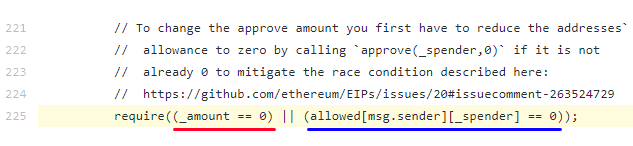
\includegraphics[width=1.0\linewidth]{figures/multiple_withdrawal_06.png}
	\caption{MiniMeToken added code to \textit{approve} method for allowing non-zero allowance values if it is already set to zero.}
\end{figure}
\noindent Similar to "Enforcement by User Interface (UI)", this will not prevent Bob from transferring N+M tokens. Because Alice would not be able to distinguish whether N tokens have been already transferred or not. It is more clear in the below scenario:
\begin{enumerate}
	\item Alice decides to set Bob’s allowance to 0.
	\item Bob front-runs Alice’s transaction and his allowance sets to 0 after transferring N tokens.
	\item Alice’s transaction is executed and sets Bob’s allowance to 0 (Red clause passes sanity check).
	\item Alice checks Bob’s allowance and she will find it 0, so, she can not determine whether this was because of her transaction or Bob already transferred N tokens.
	\item Alice considers that Bob has not been transferred any tokens and allows him for transferring new M tokens.
	\item Bob is able to transfer new M tokens and N+M in total.
\end{enumerate}

\subsection{MonolithDAO}
MonolithDAO Token\cite{Ref12} implements two additional functions for allowance increase or decrease. The default \textit{approve} function has additional codes to enforce owner for setting allowance to zero before non-zero values. It allows non-zero spender's allowance if it is already set to zero. The below table shows functionality of \textit{approve} method based on current spender's allowance and passed input \textit{\_value} as new allowance:
\begin{figure}[t]
	\centering
	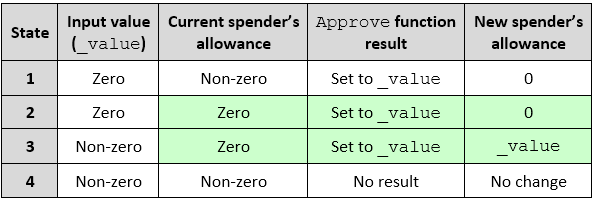
\includegraphics[width=1.0\linewidth]{figures/multiple_withdrawal_09.png}
	\caption{Functionality of default \textit{approve} method in MonolithDAO token that enforces setting spender's allowance to zero before any non-zero values. It implements ERC20 recommendation for changes allowance from N to M in two steps (N$\rightarrow$0$\rightarrow$M).}
\end{figure}
\noindent If the current spender’s allowance is non-zero, \textit{decreaseApproval}\footnote{decreaseApproval(address \textit{\_spender}, uint \textit{\_subtractedValue})} and \textit{increaseApproval}\footnote{increaseApproval(address \textit{\_spender}, uint \textit{\_addedValue})} functions have to be used for decreasing or increasing the allowance. Using these two functions can prevent race condition and mitigate the attack as explained below:
\begin{enumerate}
	\item Alice allows Bob to transfer N tokens by calling \textit{approve(\_Bob, N)}. Alice used the default \textit{approve} function consciously since current Bob’s allowance is 0. So, he checked Bob's allowance before calling \textit{approve} method.
	\item After a while, Alice decides to decrease Bob’s approval by M and runs \textit{decreaseApproval(\_Bob, M)}.
	\item Bob notices Alice’s second transaction and front runs it by executing \textit{transferFrom(\_Alice, \_Bob, N)}.
	\item Bob’s transaction will be executed first and transfers N token to his account and the his allowance becomes 0 as result of this transfer.
	\item Alice’s transaction is mined after Bob’s transaction and tries to decrease Bob’s allowance by M. If Bob had already transferred more than M tokens, new Bob’s allowance becomes negative and it fails the transaction. So, the transaction does not change Bob’s remaining allowance and he would be able to transfer the rest (which is legitimate transfer since Alice has already approved it). If Bob had transferred less than M tokens, the new allowance will be applied and reduces Bob’s allowance by M.\newline
\end{enumerate}
\noindent Although these two new functions will prevent the attack, they have not been defined in the initial specifications of ERC20. Therefore, they can not be used by smart contracts that are already deployed on the Ethereum network and still call approve method for setting new allowance---and not \textit{increaseApproval} or \textit{decreaseApproval}. Moreover, ERC20 specifications does not define any increase or decrease of allowance. It only allows setting new allowances without adjustment. For example, if Alice has approved Bob for 100 tokens and wants to set it to 80, the new allowance should be 80 while using decrease methods will set it 20 (100 - 80 = 20). Comparatively, increase method will set new allowance to 180 while it has to set it to 80 again to be in-compliant with ERC20 specification. For these reasons, this solution would not be compatible with ERC20 standard and only is usable if approver or smart contract are aware of these supplementary methods.

\subsection{Alternate approval function}
Another suggestion\cite{Ref16} is to move security checks to another function called \textit{safeApprove}\footnote{safeApprove(address \textit{\_spender}, uint256 \textit{\_currentValue}, uint256 \textit{\_value})} that compare current and new allowance values and sets it if has not been already changed. By using this function, Alice uses the standard \textit{approve} function to set Bob’s allowance to 0 and for new approvals, she has to use \textit{safeApprove} function. \textit{safeApprove} takes the current expected approval amount as input parameter and calls \textit{approve} method if previous allowance is equal to the current expected approval. By using this function, Alice will have one step more to read the current allowance and pass it to the new \textit{safeApprove} method. Although this approach mitigates the attack by using CAS pattern\cite{Ref06}, however, it is not backward compatible with already implemented smart contracts due to their unawareness of this new complementary function. In other words, the new \textit{safeApprove} method is not defined in ERC20 standard and existing smart contracts would not be able to use this new safety feature.

\subsection{Detecting token transfers}
In order to set new allowance atomically, tracking of transferred tokens is required to detect token transfers before setting new allowances. If \textit{approve} method reveals any transferred tokens due to front running, it throws an exception without setting new allowance. As suggested by \cite{Ref17}, a flag can be used to detect whether any tokens have been transferred or not. \textit{transferFrom} method sets this flag to \textit{true} in case of any token transfer. \textit{approve} method checks the flag to be \textit{false} before allowing new approvals. This approach requires new data structure to keep track of used/transferred tokens for each spender. It can prevent race condition as described below:
\begin{enumerate}
	\item Alice runs \textit{approve(\_Bob, N)} to allow Bob for transferring N tokens. Since Bob’s initial allowance is 0 and his corresponding flag=\textit{false}, then sanity check passes and Bob’s allowance sets to N in line 15.
	\item Alice decides to set Bob’s allowance to 0 by executing \textit{approve(\_Bob, 0)}.
	\item Bob front-runs Alice’s transaction and transfers N tokens. Then, \textit{transferFrom} turns his flag to \textit{true}.
	\item Alice’s transaction is mined and passes sanity check because passed value is 0.
	\item Bob’s allowance is set to 0 while his flag remains \textit{true}. (\textit{approve} method does not flip spender flags.)
	\item Alice wants to change Bob’s allowance to M by executing \textit{approve(\_Bob, M)}. Since Bob already transferred N tokens (his flag=\textit{true}), the transaction fails.
	\item Bob’s allowance does not change and he cannot move more tokens than initially allowed.\newline
\end{enumerate}
\noindent Although this approach mitigates the attack, it prevents any further legitimate approvals as well. Considering a scenario that Alice rightfully wants to increase Bob’s allowance from N to M (two non-zero values). If Bob had already transferred number of tokens, Alice would not be able to change his approval. Because Bob's flag is set to \textit{true} and line 15 does not allow changing allowance by throwing an exception:
\begin{figure}[t]
	\centering
	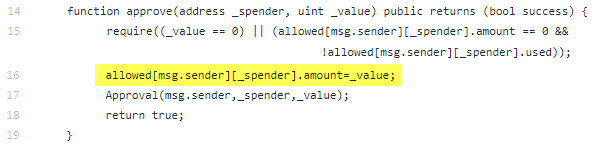
\includegraphics[width=1.0\linewidth]{figures/multiple_withdrawal_33.png}
	\caption{\textit{approve} method needs to be modifed by adding a line of code like \textit{allowed[msg.sender][\_spender].used = false;} between lines 16 and 17 to unlock spender flag for the next legitimate change.}
\end{figure}
\noindent Even setting allowance to 0 and then to M, does not flip the flag to \textit{false} (There is no code for it in the \textit{approve} method). So, It keeps Bob’s allowance locked down and blocked further legitimate allowances. In fact, \textit{approve} method needs a new code between lines 16 and 17 to set the flag to \textit{false}. But it will cause another problem. After setting allowance to 0, spender flag becomes \textit{false} and allows non-zero values event if tokens have been already transferred. It resembles the initial state of allowance similar when nothing was transferred. For example, considering front-running by Bob, before new allowance change from N to 0 by Alice. Bob's flag turns to \textit{true} by \textit{transferFrom} method and turns to \textit{false} by \textit{approve} method afterwards. Now if Alice wants to set allowance from 0 to M, Bob's flag is \textit{false} and his allowance is zero. This is similar to the situation that he did not transfer any tokens. So, Alice cannot distinguish whether Bob moved any token or not. Setting new allowance will allow Bob to transfer more tokens than Alice wanted. Therefore, adding new code makes attack mitigation functionality ineffective. In short, this approach can not satisfy both legitimate and non-legitimate scenarios. Nevertheless, it is a step forward by introducing the need for a new variable to track transferred tokens.

\subsection{Keeping track of remaining tokens}
This approach\cite{Ref18} is inspired by the previous solution and keeping track of remaining tokens instead of detecting transferred tokens. It uses modified version of data structure that used in the previous solution for storing residual tokens:
\begin{figure}[t]
	\centering
	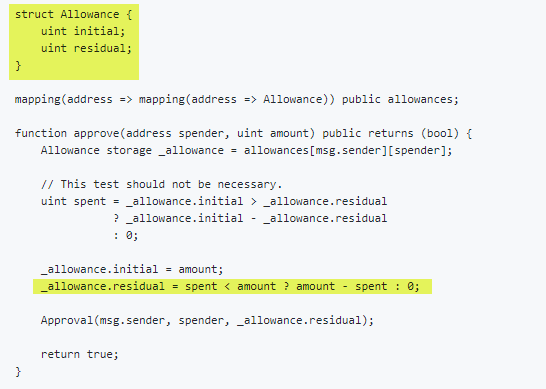
\includegraphics[width=0.9\linewidth]{figures/multiple_withdrawal_29.png}
	\caption{Keeping track of remaining tokens.}
\end{figure}
\noindent At first, it seems to be a promising solution by setting approval to zero before non-zero values. However, the highlighted code in \textit{approve} method resembles the situation that we explained in "Enforcement by User Interface (UI)". It would not be possible for Alice to distinguish if any token transfer have occurred when changing allowance. To make it more clear, considering the below scenario:  
\begin{enumerate}
	\item Bob’s allowance is initially zero (\textit{allowances[\_Alice][\_Bob].initial=0}) and his residual is zero as well (\textit{allowances[\_Alice][\_Bob].residual=0}).
	\item Alice allows Bob to transfer N tokens that makes \textit{allowances[\_Alice][\_Bob].initial=N} and \textit{allowances[\_Alice][\_Bob].residual=N}.
	\item Alice decides to change Bob’s allowance to M and has to set it to zero before any non-zero values.
	\item Bob noticed Alice’s transaction for setting his allowance to zero and transfers N tokens in advance. Consequently, \textit{transferFrom} function sets his residual to zero (\textit{allowances[\_Alice][\_Bob].residual=0}).
	\item Alice’s transaction for setting Bob's allowance to zero is mined and sets \textit{allowances[\_Alice][\_Bob].initial=0} and \textit{allowances[\_Alice][\_Bob].residual=0} This is similar to step 1 that no token has been transferred. So, Alice would not be able to distinguish whether any token have been transferred or not.
	\item Considering no token transfer by Bob, Alice approves Bob for spending new M tokens.
	\item Bob is able to transfer new M tokes in addition to initial N tokens.\newline
\end{enumerate}
Someone may think of using \textit{Transfer} event to detect transferred tokens or checking approver balance to see any transferred tokens. As explained in "Enforcement by User Interface (UI)", using \textit{Transfer} event is not sufficient in case of transferring tokens to a third party. Checking approver balance also would not be an accurate way if the contract is busy and there are lot of transfers. So, it would be difficult for the approver to detect legitimate from non-legitimate tokens transfers. Overall, this approach cannot prevent the attack.

\subsection{Changing ERC20 API}
As advised by \cite{Ref03}, changing ERC20 API could secure \textit{approve} method by comparing current allowance of the spender and sets it to new value if it has not already been transferred any tokens. This allows atomic compare and set of spender allowance to make the attack impossible. So, it will need new overloaded \textit{approve} method with three parameters in addition to the standard \textit{approve} method with two parameters:
\begin{figure}[t]
	\centering
	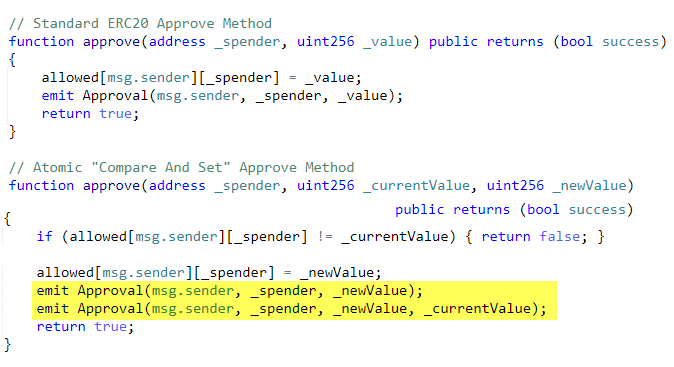
\includegraphics[width=1.0\linewidth]{figures/multiple_withdrawal_12.png}
	\caption{Suggested ERC20 API Change by adding new \textit{approve} method with three parameters to compare and set new allowance atomically.}
\end{figure}
\noindent In order to use this new method, smart contracts have to update their codes to provide three parameters instead of current two, otherwise any \textit{approve} call will use the standard vulnerable version. Moreover, one more call is required to read current allowance and pass it to the new \textit{approve} method. New event definition needs to be added to ERC20 API to log an approval events with four arguments. For backward compatibility reasons, both three-arguments and new four-arguments events have to be logged. All of these changes makes this token contract incompatible with already deployed smart contracts.

\subsection{New token standards}
After recognition of this security vulnerability, new standards like ERC233 \footnote{https://github.com/Dexaran/ERC223-token-standard}, ERC721\footnote{https://github.com/ethereum/EIPs/blob/master/EIPS/eip-721.md} and ERC777\footnote{https://eips.ethereum.org/EIPS/eip-777} were introduced to address the issue in addition to improving current functionality of ERC20 standard. They changed approval model and fixed some drawbacks which need to be addressed in ERC20 as well (i.e., handle incoming transactions through a receiver contract, lost of funds in case of calling \textit{transfer} function instead of \textit{transferFrom}, etc). Nevertheless, migration from ERC20 to ERC223/ERC721/ERC777 would not be convenient and all deployed ERC20 tokens (168,092\footnote{https://etherscan.io/tokens} tokens as of 18 February 2019) needs to be redeployed. This also means update of any trading platform listing ERC20 tokens. The goal here is to find a backward compatible solution instead of changing current ERC20 standard or migrating tokens to a new standards. Despite expanded features and improved security properties of new standards, we would not consider them as target solutions.